\chapter{BAYESIAN ESTIMATION OF SUBSET THRESHOLD AUTOREGRESSIVE MODELS FOR SHORT-TERM FORECASTING OF TRAFFIC OCCUPANCY}
\label{chap:traffic}
%%%%%%%%%%%%%%%%%%%%%%%%%%%%%%%%%%%%%%%%%%%%%%%%%%%%%%%%%%%%%%%%%%%%%%%
\section{Introduction}
Rising populations in major cities add stress to advanced traffic management systems (ATMS) tasked with monitoring real-time traffic variables to proactively reduce congestion. Ever since \cite{Ahmed1979} used basic ARIMA strategies to model freeway traffic networks in large US cities -- Los Angeles, Minneapolis, and Detroit -- significant research has accumulated to appropriately utilize the massive amount of data obtained in transportation networks. The global concern has manifested through independent research in major cities in places such as the United Kingdom \citep{Queen2009,Dunne2012}, Greece \citep{Stathopoulos2003, Kamarianakis2012,Theofilatos2017}, Italy \citep{Annunziato2013,Moretti2015}, China \citep{Shang2006,Jun2007,Min2010}, and Ethiopia \citep{Hellendoorn2011}. Technological advances over this time period have not only improved the gathering of the data but also in the quick distribution of pertinent information to drivers. The speed and accuracy between the detection to the correction rely on efficient modeling and accurate short-term forecasting of important traffic characteristics.

Three traffic variables have been used to quantify traffic congestion per unit of time: flow (volume per time), speed (distance per time), and occupancy (percent of time occupied) \cite{Hall1992}. \cite{Smith1997} provide insight into the state of traffic modeling 20 years ago while \cite{Vlahogianni2014} do an excellent job summarizing recent advancements in short-term traffic forecasting by posing 10 interesting challenges for future researchers. The scarcity of forecast procedures for traffic occupancy may stem from the instability acknowledged in \cite{Levin1980}. Traffic occupancy, the percent of time a detection zone is occupied, has been described as ``quality assessment measure'' as it quantifies how well traffic is moving through a network \citep{Klein1996}. Univariate approaches for modeling traffic occupancy are presented for the terminal goal of evaluating forecasts at multiple horizons. Section \ref{sec:trafficdata}  presents a challenging traffic dataset from a major arterial in Athens, Greece, used for empirical study.

Traffic occupancy has been used to help forecast other traffic characteristics \citep{Hazelton2004}.  In regards to modeling traffic occupancy, most researchers adapt similar methods seen for traffic flow and speed \citep{Kamarianakis2010}. Like other traffic variables, occupancy exhibits abrupt changes in mean, temporal dynamics, and volatility as traffic fluctuates between free flow and congested states. Realizations of recent traffic occupancy can assist in the characterization of these states. In Section \ref{sec:trafficmodels}, nonlinear threshold autoregressive (TAR) processes  model and forecast traffic occupancy. The parametric TAR structure, first discussed in \cite{Tong1990}, is a conditional autoregressive (AR) model dependent on states governed by traffic occupancy . The model is highly interpretable making it appealing to practitioners. For easy application, TAR models for each location are defined to be day-specific and horizon-specific. Also, a periodic linear regression model that adequately captures the seasonality exhibited in traffic data is used to produce baseline forecasts.

\cite{Ghosh2007} provide a case for the movement from classical inference to Bayesian inference in traffic models. Joint contributions from \cite{Broemeling1992,Geweke1993,Chen1995} formed the foundation of Bayesian TAR modeling. \cite{Campbell2004} applied reversible jump Markov chain Monte Carlo to select regime-specific AR orders. Subset selection of TAR via stochastic search variable selection \citep{George1993} was conducted by \citet{So2003,Chen2011}. For all the aforementioned approaches, the number of regimes must be known or assumed. In illustration, simulation, and application, TAR models are often restricted to have at most three regimes. 

\cite{Chan2015} transformed the nonlinear TAR model into a high dimensional linear regression. Multi-step procedures seek sparse solutions to identify the regimes and perform parameter estimation \citep{Chan2015,Chan2017}. The fully Bayesian approach of \cite{Pan2017} operates similarly by utilizing a sequence of binary inclusion variables to identify change points and select regimes. The fully saturated TAR model defined Section \ref{sec:trafficmodels} follows from \cite{Chan2015} with some slight modifications. 

Section \ref{sec:trafficest} proposes a fully Bayesian three step  procedure that automates selecting the regimes and sparse subset AR estimation within regimes. First, a fully saturated TAR model is estimated using Bayesian regularization implemented through a modified horseshoe prior \citep{Carvalho2009,Carvalho2010,Bhadra2016}. Next, the Kullback-Leibler (KL) divergence \citep{Kullback1951} combined with a forward selection algorithm identifies the regimes through comparing posterior predictive distributions of the linear AR model to multiple regime TAR models. Finally, given a restricted set of regimes, the same procedure is repeated to select the relevant dynamics within each of the regimes. The result is a parsimonious TAR model with a posterior predictive distribution close in KL distance to the posterior predictive distribution from the full model.

Section \ref{sec:trafficresults} provides empirical results of out-of-sample forecasting results from final TAR models with potentially many regimes. Baseline periodic seasonal regressions are used to produce baseline forecasts. Models are compared using the mean absolute scaled measure of forecast accuracy (MASFE) of \cite{Hyndman2006}. By scaling forecast errors by the mean absolute error from a horizon-specific naive random walk, models can be simultaneously be compared to each other and the naive method.






%%%%%%%%%%%%%%%%%%%%%%%%%%%%%%%%%%%%%%%%%%%%%%%%%%%%%%%%%%%%%%%%%%%%%%%
\section{Data}
\label{sec:trafficdata}

Real-time traffic data are obtained from the major Athen's arterial, Alexandras Avenue, along the westbound direction. Every 90 seconds in April 2000, traffic occupancy is captured from seven loop detectors abbreviated $L \in \{A,B,C,D,E,F,G\}$. The National Technical University of Athens is credited for the gathering of this data. The 2013 Traffic Research Board's (TRB) Annual Meeting Workshop used a larger ecompassing dataset in their TRANSportation Data FORecasting Competition (TRANSFOR). This competition was organized by the Aritificial Intelligence and Advanced Computing Applications Committee.  Many of the inherent characteristics in this dataset make short-term forecasting quite challenging. The winning methodology applied adaptive lasso to high-dimensional nonlinear space-time models \citep{Kamarianakis2012}. Figure \ref{fig:trafficdatamap} was created using Google Maps to provide a visual depiction of this small network with arrows representing direction of traffic flow. Loop detectors $A$, $B$, $C$, and $D$ measure traffic occupancy in the westbound direction, and detectors $E$, $F$, and $G$, in the eastbound direction.

\begin{figure}[htbp]
\caption{Locations of Loop Detectors Along Alexandras Ave. in Athens, Greece: Arrows Indicate Direction of Traffic Flow}
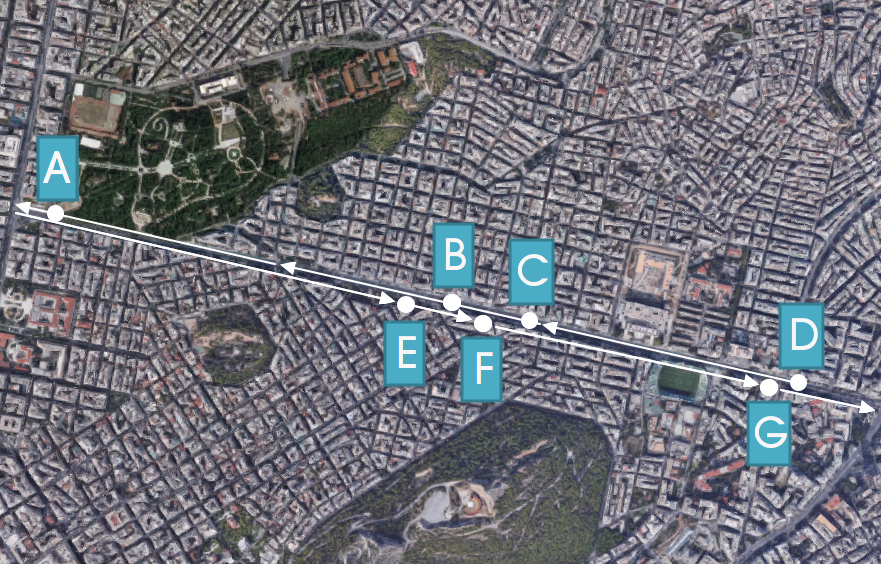
\includegraphics[width=\textwidth]{TrafficMap2}
\label{fig:trafficdatamap}
\end{figure}

Analyzing the raw traffic occupancy from an urban network measured on the 90s interval becomes problematic due to the large amount of noise seen at high resolutions \citep{Vlahogianni2014}. Temporal aggregation to larger intervals i.e. 15 min has been practiced over the years as a smoothing technique prior to modeling. Not only does this practice make short-term forecasting irrelevant with today's technology but diminishes useful long memory, nonlinear, and heteroskedastic dynamics in the underlying signal \cite{Vlahogianni2011}.Rather than modeling across different levels of temporal aggregation, as seen in \cite{Shang2006}, traffic occupancy is averaged to 3 minute intervals resulting in 480 daily time points per location. 

Define random variable $O_{L,t}$ as the traffic occupancy for location $L$ at time $t$ and $o_{L,t}$ represents a known realization. As common practice, weekend data is ignored. Cyclical human behavior patterns throughout the work week lead to weekly seasonal traffic patterns. Data during April 2000 covers four complete weeks. The first three weeks are used to fit TAR models, and the last week is designated for forecasting evaluation. Time series plots of $\{o_{L,t}\}$ are found in Figure \ref{fig:OrigPlotTrafficOcc} organized by location.

\begin{figure}[htbp]
\caption{Raw Traffic Occupancy for All Locations Measured on 3-Minute Interval: Shaded Region Indicates the Forecasting Period}
\includegraphics[width=\textwidth]{rawplots}
\label{fig:OrigPlotTrafficOcc}
\end{figure}







%%%%%%%%%%%%%%%%%%%%%%%%%%%%%%%%%%%%%%%%%%%%%%%%%%%%%%%%%%%%%
\section{Threshold Autoregressive Model}
\label{sec:trafficmodels}

\subsection{General Modeling Information}
For each location $L\in \{A,B,C,D,E,F,G\}$, day of the week $D\in\{M,T,W,Th,F\}$, and horizon $h \in \{1,3,5\}$ ,  $(L,D,h)$-specific TAR models are built to forecast $\widehat{O}_{L,t}=E[O_{L,t}|\mathcal{I}_t]$ where $\mathcal{I}_t=\{o_{L,k}\}_{k=t-h}^{t-h-P+1}$. Chosen horizons correspond to 3 min, 9 min, and 15 min ahead forecasts. The weekly periodicity of traffic occupancy modeled in \cite{Williams1999,Ghosh2007,Kamarianakis2010} and visually seen in Figure \ref{fig:OrigPlotTrafficOcc} defends $D$-specific modeling. The purpose of $h$-specific models is to ensure multi-step forecasting is user-friendly and computationally efficient for practitioners. 

The order parameter $P\in\mathbb{N}$ represents the maximum short-term lag relevant for forecasting and should be chosen large enough to cover relevant temporal dependencies across all traffic states. The order $P=7$ is fixed equating to the last 21 minutes of known information. To produce short-term forecasts, only short-term dynamics are considered. Long-term or seasonal dynamics can be included but require more periods to adequately estimate. Periodic regression models with Fourier terms adequately capture weekly seasonality and are used to produce baseline forecasts \citep{Kamarianakis2010}. As $h\to\infty$, $(L,D)$-specific seasonal models are expected to dominate over $(L,D,h)$-specific TAR models.
 
\subsection{Transformed Occupancy}
Using function $\textrm{logit}(x):(0,1)\to\mathbb{R}$ such that $\phi(x)=\log [x/(1-x)]$, define the new transformed variable $Y_{L,t}=\textrm{logit}(O_{L,t})$. Raw occupancy is bounded on the $[0,1]$ interval. Recoding $0$ with $0.0001$ and $1$ with $0.9999$ is a nonevasive technique to handle extreme occupancies when $\textrm{logit}(.)$ is undefined. All models are defined for the variable $Y_{L,t}$, an approach used for proportional time series since \cite{Wallis1987}. Figure \ref{fig:TransPlotTrafficOcc} displays the transformed series $\{y_{L,t}\}$ for each location. Although forecasts are produced for the final week, evaluation of forecasts are considered on the original scale using $\textrm{logit}^{-1}(x):\mathbb{R}\to(0,1)$ where $\textrm{logit}^{-1}(x)=\frac{\exp(x)}{1+\exp(x)}$. Since $\textrm{logit}(x)$ is a nonlinear transformation, the forecast $\hat{O}_{L,t} \neq  \textrm{logit}^{-1}(\hat{Y}_{L,t})$. Unbiased forecasts and quantiles are produced from the set $\{\textrm{logit}^{-1}(\hat{Y}^{(s)}_{L,t})\}_{s=1}^{S}$ where $\{\hat{Y}^{(s)}_{L,t}\}_{s=1}^{S}$ are $S$ posterior samples obtained from the posterior predictive distribution $f(\hat{Y}_{L,t}|\mathcal{I}^*_t)$ where $\mathcal{I}^*_t=\{y_{L,k}\}_{k=t-h}^{t-h-P+1}$.
\begin{figure}[htbp]
\caption{Logit Transformed Traffic Occupancy for All Locations Measured on 3-Minute Interval: Shaded Region Indicates the Forecasting Period}
\includegraphics[width=\textwidth]{Transplots}
\label{fig:TransPlotTrafficOcc}
\end{figure}

\subsection{General $(L,D,h)$-Specific TAR Model}
The random process $\{Y_t\}$ follows TAR model of order $P$ with $m+1$ regimes if 
\begin{equation}
\label{eq:generalTAR}
Y_{t}=\phi_0^{(j)}+\sum\limits_{i=1}^P \phi^{(j)}_i Y_{t-h-i+1}+\sigma\epsilon_{t}, \textrm{ for } \delta_{j-1}<Y_{t-h}\leq \delta_{j},
\end{equation}
where $\sigma>0$, $j\in\{1,2,\cdots,m+1\}$, and $h \in \mathbbm{N}$. The vector of thresholds $\bm{\delta}=[\delta_1,\delta_2,\cdots,\delta_m]'$ divides the process into $m+1$ regimes where $-\infty=\delta_0<\delta_1\leq\delta_2\leq \cdots \leq \delta_m<\delta_{m+1}=\infty$. Since the most recent realization $Y_{t-h}$ determines the current model state, the TAR model is conventionally classified as ``self-exciting" \citep{Ghaddar1981}. The sequence of errors $\{\epsilon_t\}$ are assumed to be i.i.d. with zero mean and unit variance.

The TAR structure in Equation \ref{eq:generalTAR} is slightly more rigid than the classic structure in \cite{Chen1995}. Rather than utilizing regime-specific variance parameters $\sigma_j$,  homoskedasticity is assumed. When $\textrm{logit}^{-1}(x)$ is used to obtain density forecasts on the original $[0,1]$ scale, heteroskedasticity is naturally captured. This is analogous to \textit{Beta} distributed random variables where the variance is dependent on the mean. Another key difference arises in the selection of the transition variable. Often a delay parameter $d$ is introduced and $Y_{t-d}$ drives regime changes. Following from \cite{Chan2015}, $d$ is known and  $d=h$ is fixed. Exogenous traffic variables nor time are considered for the transition variable.

\subsection{High Dimensional Linear Representation}
To reformulate Equation \ref{eq:generalTAR} into a high dimensional linear regression model, a slight deviation from the procedure in \cite{Chan2015,Chan2017} is outlined with similar notation for consistency. Suppose the discrete time series $\{y_t\}_{t=1-h-P+1}^T$ is observed. Let $\bm{y}=[y_{1},\cdots,y_{T}]'$, $\bm{\epsilon}=[\epsilon_{1},\cdots,\epsilon_{T}]'$, and define matrix $\bm{X}$ by
$$
\bm{X}=\begin{bmatrix}
    1 & y_{1-h} & y_{1-h-1} & \dots  & y_{1-h-P+1} \\
    1 & y_{2-h} & y_{2-h-1} & \dots  & y_{2-h-P+1} \\
    \vdots & \vdots & \vdots & \ddots & \vdots \\
    1 & y_{T-h} & y_{T-h-1} & \dots  & y_{T-h-P+1}
\end{bmatrix}.
$$
The $T\times 1$ response vector $\bm{y}$, $T\times 1$ error vector $\bm{\epsilon}$, and  $T \times (1+P)$ model matrix $\bm{X}$ are often seen in matrix representations of $h$-specific AR$(P)$ models.

The second column in $\bm{X}$ contains the sequence of $h$-specific transition variables. Define the sorting function $\pi(i):\{1,\cdots,T\}\to\{1,\cdots,T\}$   where $\pi(i)$ equates to the time index of the $i$th smallest element in $[y_{1-h},y_{2-h},\cdots,y_{T-h}]'$. The new $\bm{y}_R=[y_{\pi(1)+h},\cdots,y_{\pi(T)+h}]'$, $\bm{\epsilon}_R=[\epsilon_{\pi(1)+h},\cdots,\epsilon_{\pi(T)+h}]'$ and 
$$
\bm{X}_1=\begin{bmatrix}
    1 & y_{\pi(1)} & y_{\pi(1)-1} & \dots  & y_{\pi(1)-P+1} \\
    1 & y_{\pi(2)} & y_{\pi(2)-1} & \dots  & y_{\pi(2)-P+1} \\
    \vdots & \vdots & \vdots & \ddots & \vdots \\
    1 & y_{\pi(T)} & y_{\pi(T)-1} & \dots  & y_{\pi(T)-P+1}
\end{bmatrix}=
\begin{bmatrix}
\bm{y}'_{\pi(1)} \\
\bm{y}'_{\pi(2)} \\
\vdots \\
\bm{y}'_{\pi(T)} \\
\end{bmatrix}
$$
are essentially $\bm{y}$, $\bm{\epsilon}$, and $\bm{X}$ sorted according to the order statistics of the transition variable. The reordered errors in $\bm{\epsilon}_R$ are assumed to be i.i.d. with mean $0$ and variance $\sigma^2$.

In practical application, it makes sense to limit the TAR model to $m+1$ regimes requiring the estimation of $m$ thresholds in the range of the transition variable. Let $q(.): [0,1]\to[\min\{y_{t-h}:t=1,2,\cdots,T\},\max\{y_{t-h}:t=1,2,\cdots,T\}]$ denote the sample quantile function and consider a sequence $\{p_k\}_{k=1}^m$ of $m$ evenly spaced percentiles such that $p_{min}=p_1<\cdots<p_m=p_{max}$. For a fully saturated TAR model limited to $(m+1)$ regimes, fix \textit{a priori} the vector of thresholds $\bm{\delta}=[q(p_{1}),q(p_2),\cdots,q(p_{m})]'$. For $j \in \{2,\cdots,m+1\}$, let $k_j$ represent the number of elements in $[y_{1-h},y_{2-h},\cdots,y_{T-h}]'$ less than $q(p_{j-1})$ and  define 
$$\bm{X}_j=
\begin{bmatrix}
    0 & 0 & 0 & \dots  & 0 \\
    \vdots & \vdots & \vdots & \ddots & \vdots \\
    0 & 0 & 0 & \dots  & 0 \\
    1 & y_{\pi(k_j+1)} & y_{\pi(k_j+1)-1} & \dots  & y_{\pi(k_j+1)-P+1} \\
    \vdots & \vdots & \vdots & \ddots & \vdots \\
    1 & y_{\pi(T)} & y_{\pi(T)-1} & \dots  & y_{\pi(T)-P+1}
\end{bmatrix}=
\begin{bmatrix}
0 \\
\vdots \\
0\\
\bm{y}'_{\pi(k_j+1)} \\
\vdots \\
\bm{y}'_{\pi(T)} \\
\end{bmatrix}.
$$

Finally, a slightly restricted version of the $(m+1)$-regime TAR process seen in Equation \ref{eq:generalTAR} can be expressed as a linear regression by
\begin{equation}
\label{eq:hdlinmod}
\begin{split}
\bm{y}_R &=\bm{X}_R\bm{\theta}_R+\bm{\epsilon}_R \\
\end{split}
\end{equation}
where $\bm{X}_R=[\bm{X}_1,\bm{X}_2,\cdots,\bm{X}_{m+1}]$ is a $T\times (P+1)(m+1)$ model matrix and $\bm{\theta}_R=[\bm{\theta}'_{1},\bm{\theta}'_2,\cdots,\bm{\theta}'_{m+1}]'$ is a $(P+1)(m+1) \times 1$ vector of coefficients grouped by regime. From Equation \ref{eq:generalTAR}, set $\bm{\phi}_j=[\phi^{(j)}_0,\phi^{(j)}_1,\cdots,\phi^{(j)}_P]'$. Starting with $\bm{\theta}_1=\bm{\phi}_1$, the state dependent coefficient group $\bm{\theta}_j=\bm{\phi}_{j}-\bm{\phi}_{j-1}$ for $j \in \{2,\cdots,m+1\}$ represents the marginal adjustment in dynamics when $y_{t-h}$ crosses the threshold $\delta_{j-1}=q(p_{j-1})$.

\subsection{Baseline Seasonal Model}
Seasonal models allow us to understand the long-run relationship of a variable over time through repetitive cycles. It is common practice in time series analysis to deseasonalize data prior to model buiding through smoothing or seasonal differencing. In many studies, seasonal autoregressive integrated moving average models (SARIMA) have been used to analyze traffic characteristics \citep{Williams2003, Ghosh2005, Zhang2011}. As detailed in \cite{Kumar2015}, these models require large databases of historical data to capture seasonal phenomenon. Similar to \cite{Kumar2015}, a 3 day period is used for model training. From a similar dataset, \cite{Kamarianakis2010} used a smoothing spline with 150 degrees of freedom to magnify weekly seasonal patterns and identify structural changes. Smoothing approaches can lead to simple models that can forecast at all horizons.

Harmonic regressions estimate daily periodic signals from a linear regression over a Fourier basis \citep{Metcalfe2009}. For 3-min data, the seasonal period has a length of 480 discrete measures. Using harmonic regression, $(L,D)$-specific seasonal profiles of $\{Y_t\}$ are fitted. Expressed in Equation \ref{eq:trafficseas}, the harmonic seasonal model is restricted to the first $H$ terms of the Fourier series.  This model is not considered a baseline model for its simplicity in estimation but for its simplicity in multi-step forecasting at all horizons. The error $\{\epsilon_t\}$ are assumed i.i.d. with mean 0 and unit variance.
\begin{equation}
\label{eq:trafficseas}
Y_{t}=\mu+\sum\limits_{j=1}^{H} \Big[\alpha_{j}\sin\Big(\frac{2\pi tj}{480}\Big)+\beta_{j}\cos\Big(\frac{2\pi tj}{480}\Big)\Big]+\sigma\epsilon_{t}
\end{equation}

Fitting the model in Equation \ref{eq:trafficseas} is not difficult since it can also be represented as a high dimensional linear regression model like
\begin{equation}
\label{eq:hdslinmod}
\begin{split}
\bm{y}_F &=\bm{X}_F\bm{\theta}_F+\bm{\epsilon}_F \\
\end{split}
\end{equation}
where $\bm{y}_F=[y_1,y_2,\cdots,y_T]'$, $\bm{\epsilon}_F=[y_1,y_2,\cdots,\epsilon_T]'$, and $\bm{\theta}_F=[\mu,\alpha_1,\cdots,\alpha_H,\beta_1,\cdots,\beta_H]'$. The model matrix  $\bm{X}_F=[\bm{1},\bm{SIN},\bm{COS}]$ where $\bm{1}$ is a $T\times 1$ vector of $1$s, $\bm{SIN}$ is a $T\times H$ matrix containing the Fourier sine terms, and $\bm{COS}$ is a $T\times H$ matrix containing the Fourier cosine terms.

\subsection{Special Considerations for Traffic Modeling}
The linear matrix form of TAR in Equation \ref{eq:hdlinmod} arises from restricting the set of possible thresholds  $\bm{\delta}$ to a finite set of quantiles based on the sampled transition variable. The high dimensional regression model in \cite{Chan2015,Chan2017} represents a fully saturated TAR model where every realization in the series $\{y_t\}_{t=1}^T$ resides in a different regime. In classic Bayesian handling of TAR and the related smooth transition autoregressive model (STAR), the number of regimes, $(m+1)$, is fixed. To restrict estimation of the $m$ thresholds to the range of $Y_{t-h}$, slightly informative \textit{uniform} priors bounded by empirical quantiles $q(p_{min})$ and $q(p_{max})$ ensure that at least $(1-\min\{p_{min},1-p_{max}\})\times 100\%$ of the data is represented in the lowest and highest regime \citep{Chen1995,Chen1998,Lubrano2000,Lopes2006}. Following from literature, $p_{min}=0.15$ and $p_{max}=0.85$ are selected to slightly reduce the dimensionality of $\bm{X}$.

For $(L,D,h)$-specific traffic models, the maximum number of thresholds is fixed to $m=50$ and the maximum autoregressive order to $P=7$. The model matrix $\bm{X}_R$ of the fully saturated $51$-regime TAR$(7)$ has dimension $T^*\times 408$. The fitting period for each model contains $T=1440$ discrete time realizations of $\{Y_t\}$ leading to $T^*=1440-h-7+1 > 408$. The predetermined threshold vector $\bm{\delta}=[q(0.15),q(p_2),\cdots,q(p_{49}),q(0.85)]'$ constructed from $m$ evenly spaced percentiles ensures approximately $\frac{0.85-0.15}{50}=0.014$ of the full time series is represented in each potentially relevant regime. These modifications to the framework of \cite{Chan2015,Chan2017} are made to ensure the dimensionality of the parameter space is not unnecessarily large for practical application. Based on this approach, it is recommended to select $m$ large enough to ensure the set of quantile-based thresholds is dense to not reduce error in misspecified \textit{a priori} selection of $\bm{\delta}$.

For $(L,D)$-specific seasonal models, the number of Fourier sine/cosine pairs $H$ must be less than half the period. Regularized estimation of these models using adaptive LASSO \citep{Zou2006} indicated that the largest significant harmonic of the model in Equation \ref{eq:trafficseas} across locations and days was for $j=139$. Before estimating these seasonal profiles under the Bayesian framework, a maximum number of harmonics, $H=150$, is chosen. The vector of coefficients $\bm{\theta}_F$ contains $2H+1=301<1440=T$ parameters that require estimation. To ensure weekly periodic signals are smooth, sparse estimation of $\bm{\theta}_F$ is desired.








%%%%%%%%%%%%%%%%%%%%%%%%%%%%%%%%%%%%%%%%%%%%%%%%%%%%%%%%%%%%
\section{Bayesian Estimation, Regime Identification, and Subset Selection}
\label{sec:trafficest}

The purpose of representing the $(m+1)$-regime TAR process as a high dimensional linear regression is to make Bayesian posterior estimation and model selection computationally feasible for multiple regime TAR models. More importantly, the fully saturated regression $\bm{y}_R=\bm{X}_R\bm{\theta}_R+\bm{\epsilon}_R$ nests a finite, but extensive, library of $(m^*+1)$-regime subset TAR$(P)$ models where $0\leq m^*\leq m$. This includes all linear subset AR$(P)$ models.

For simplicity, let $\bm{\Theta}=[\bm{\theta}'_R,\sigma^2]'=[\bm{\theta}'_1,\cdots,\bm{\theta}'_{m+1},\sigma^2]'$. It is believed that the optimal choice $m^*$ is small implying that only $m^*+1$ of the vectors in $\{\bm{\theta}'_1,\bm{\theta}'_2,\cdots,\bm{\theta}'_{m+1}\}$ are nonzero implying that $\bm{\theta}_R$ is sparse. To simultaneously estimate $\bm{\theta}_R$, choose the optimal $m^*$, and identify the thresholds, \cite{Chan2015} recommends using the penalized group LASSO estimate $\hat{\bm{\theta}}_{GL}$ of \cite{Yuan2006} seen in Equation \ref{eq:grouplasso}. The parameter $\lambda$ controls regularization, $||\cdot||_2$ is the $\ell_2$-norm, and $||\cdot||_1$ is the $\ell_1$-norm.
\begin{equation}
\label{eq:grouplasso}
\hat{\bm{\theta}}_{GL}=\underset{\bm{\theta}_R}{\textrm{argmin}}=\frac{1}{T}||\bm{y}_R-\bm{X}\bm{\theta}_{R}||_2^2+\lambda\sum\limits_{j=1}^{m+1}||\bm{\theta}_j||_1
\end{equation}

When $\bm{X}_R$ is constructed as seen in \cite{Chan2015},the set of thresholds identified from $\hat{\bm{\theta}}_{GL}$ consistently estimates the true thresholds if the true $m^*$ is known \textit{a priori}. In practice, $m^*$ is unknown, and $\hat{\bm{\theta}}_{GL}$ overestimates the number of regimes. Second stage selection of the best subset of the group LASSO identified thresholds via penalized information criteria (IC), i.e. AIC \citep{Li2012}, BIC \citep{Yao1988}, or MDL \citep{Davis2006}, leads to consistent estimation of the true set of thresholds \citep{Chan2015}. The three-step procedure of \cite{Chan2017}, primarily based on a group orthogonal greedy algorithm (GOGA) and high dimensional information criteria (HDIC), significantly outperforms two-step group LASSO approach in \cite{Chan2015}.

The estimation procedures of \cite{Chan2015,Chan2017} focus on estimation and selection of $\bm{\delta}$ assuming $P$ is known and the same for each regime. The consistency and convergent rate maintain when these assumptions are dropped. Using the Bayesian framework, a three step procedure, outlined in Sections \ref{sec:stage1}, \ref{sec:stage2}, and \ref{sec:stage3}, identifies the important regimes with potentially subset AR$(P)$ dynamics. The order parameter $P$ should be chosen large enough to cover all temporal dynamics across all regimes, and, as previously mentioned, $P=7$ for all $(L,D,h)$-specific traffic occupancy subset TAR$(P)$ models.

\subsection{Bayesian Penalized Estimation}
\label{sec:stage1}

\subsubsection{Conditional Likelihood}
All Bayesian inference extends from the full posterior distribution $p(\bm{\Theta}|\bm{y}_R,\bm{X}_R)$. As Bayes' rule suggests, the full posterior distribution is expressed as
\begin{equation}
\label{eq:fullpost}
p(\bm{\Theta}|\bm{y}_R,\bm{X}_R) \propto p(\bm{y}_R|\bm{X}_R,\bm{\Theta})p(\bm{\Theta})
\end{equation}
where $p(\bm{y}_R|\bm{X}_R,\bm{\Theta})$ is the model likelihood and $p(\bm{\Theta})$ is the prior. Options for $p(\bm{\Theta})$ are discussed in the subsequent section, but all immediate attention is on the model likelihood $p(\bm{y}_R|\bm{X}_R,\bm{\Theta})$. Given the linear model $\bm{y}_R=\bm{X}_R\bm{\theta}_R+\bm{\epsilon}_R$, the likelihood $p(\bm{y}_R|\bm{X}_R,\bm{\Theta})$ stems from a distributional assumption about the errors $\{\epsilon_{\pi(t)+h}\}$ in $\bm{\epsilon}_R$. So far, we have assumed $\{\epsilon_{\pi(t)+h}\}$ are i.i.d. with mean $0$ and variance $\sigma^2$. For modeling traffic occupancy, we consider and compare two distribution options.

Assume $\{\epsilon_{\pi(t)+h}\} \sim \textrm{ i.i.d. }\mathcal{N}(0,\sigma^2)$ where $\mathcal{N}$ denotes the \textit{normal} distribution. Throughout statistics, this is the most commonly used distribution for the errors. The \textit{normal} regression model is recognized by 
\begin{equation}
\label{eq:normalmod}
\bm{y}_R|\bm{X}_R,\bm{\Theta}\sim \mathcal{N}_T(\bm{X}_R\bm{\theta}_R,\sigma^2\bm{I})
\end{equation}
where $\mathcal{N}_T$ is a $T$-dimensional \textit{Multivariate normal} distribution and $\bm{I}$ is a $T\times T$ identity matrix. The \textit{Gaussian} error specification for all $(L,D,h)$-specific TAR models and $(L,D)$-specific seasonal harmonic profiles is used with caution. Even after aggregating to a 3-min interval, influential spikes toward $0$ and $1$ are seen. For future reference, we let TAR and SEAS denote the \textit{normal} regression models from Equations \ref{eq:hdlinmod} and \ref{eq:hdslinmod}. In both TAR and SEAS, Jefferys' prior is used for $\sigma^2$. Derivation of the \textit{inverse-gamma} full conditional distribution for $\sigma^2$ under both linear models can be found in \cite{bayesreg}.

\subsubsection{Horseshoe+ Priors for Penalized Regression}

\cite{Mallick2013} examines the historical significance of Bayesian model selection approaches in high dimensional linear models. Bayesian penalized regression methods using continuous scale-mixture priors \citep{OHara2009,Polson2010} have been proposed to approximate the spike-and-slab shape of discrete mixture priors \citep{Mitchell1988,George1993,Madigan1994,Carlin1995,Kuo1998,Ishwaran2005,Ishwaran2011}.

Specifically, the Bayesian horseshoe (BHS) estimator of \citep{Carvalho2009,Carvalho2010} has been extensively researched and shown to have excellent theoretical properties in achieving sparsity \citep{Polson2012,Datta2013,vanderPas2014}. The BHS prior falls in the extensive class of shrinkage priors with global-local hierarchical representations \citep{Polson2010}. As common to regularization techniques, a global tuning parameter is used to enforce variable selection by shrinking coefficients toward 0. However, BHS utilizes additional coefficient-specific tuning parameters to ensure relevant effects are not overshrunk. 

The horseshoe+ estimator ($\textrm{BHS}^+$) of \cite{Bhadra2016} results from a slightly modified hierarchy with additional tuning on the local level. The $\textrm{BHS}^+$ hierarchical prior for each parameter $\theta_i$ in the full parameter vector $\bm{\theta}_R$ is represented as
\begin{equation}
\label{eq:traffichsp}
\begin{split}
	\theta_i|\lambda_i,\tau,\sigma^2 & \sim \mathcal{N}(0,\lambda^2_i\tau^2\sigma^2) \\
	\lambda_i &\sim \mathcal{C}^+(0,\eta_i)\\
	\eta_i & \sim \mathcal{C}^+(0,1)\\
	\tau &\sim \mathcal{C}^+(0,1)\\
\end{split}
\end{equation}
where $\mathcal{C}^+$ is the \textit{half-Cauchy} distribution. The $\textrm{BHS}^+$ prior provides better detection of ultra-sparse signals than the original BHS; therefore, $\textrm{BHS}^+$ shrinkage priors are preferred in all TAR and SEAS models.  Additional theoretical and empirical defense of $\textrm{BHS}^+$ priors in the high dimensional regression setting, see \cite{Bhadra2016} and Appendix \ref{appendix3}.

The original hierarchy seen in Equation \ref{eq:traffichsp} makes posterior sampling difficult since full conditional distributions are not obtainable. By exploiting the scale-mixture decomposition of the \textit{half-Cauchy} distribution using \textit{inverse gamma} distributions abbreviated $\mathcal{IG}$ \citep{Wand2011}, \cite{Makalic2016b} derived full conditional distributions for all parameters in $\bm{\Theta}$ so Gibbs sampling \citep{Geman1987,Gelfand1990} can be utilized to sample from the full posterior distribution $p(\bm{\Theta}|\bm{y}_R,\bm{X}_R)$. Equation \ref{eq:traffichsp2} reflects the changes to the $\textrm{BHS}^+$ hierarchy for each parameter $\theta_i$ in $\bm{\theta}_R$.
\begin{equation}
\label{eq:traffichsp2}
\begin{split}
\theta_i|\lambda_i^2,\tau^2,\sigma^2 & \sim \mathcal{N}(0,\lambda_i^2\tau^2\sigma^2) \\
\lambda^2_i|\nu_i & \sim \mathcal{IG}(1/2,1/\nu_i)\\
\nu_i|\eta_i & \sim \mathcal{IG}(1/2,1/\eta^2_i) \\
\eta^2_i|\zeta_i & \sim \mathcal{IG}(1/2,1/\zeta_i) \\
\zeta_i & \sim \mathcal{IG}(1/2,1) \\
\tau^2|\xi & \sim \mathcal{IG}(1/2,1/\xi)\\
\xi & \sim \mathcal{IG}(1/2,1) \\
\end{split}
\end{equation}

\subsubsection{Posterior Sampling}
The high dimensional TAR and SEAS models, with large $\bm{X}_R$ and $\bm{X}_F$ design matrices, causes issues in Gibbs sampling. Specifically, the full conditional distributions of $\bm{\theta}_R$ and $\bm{\theta}_S$ require large $408\times 480$ and $301\times 301$ matrices, respectively. To obtain $S$ posterior samples $\{\bm{\theta}^{(s)}_R\}_{s=1}^{S}$ and $\{\bm{\theta}^{(s)}_F\}_{s=1}^{S}$, inversion of $\bm{X}'_R\bm{X}_R$ and $\bm{X}'_S\bm{X}_S$ is required in the derived \textit{multivariate normal} full conditional distributions. In all cases, the algorithm of \cite{Rue2001} provides fast Gibbs sampling, but for larger choices of $m$, $P$, and $H$, the algorithm of \cite{Bhattacharya2016} is a helpful alternative. For both TAR and SEAS models,  $S=2000$ posterior samples after a burn-in period of $5000$ and with a thinning of $10$ was large enough to ensure the minimum effective sample size of all parameters was larger than $150$. Posterior means and quantiles capture the uncertainty of the models given the data. Even though $\textrm{BHS}^+$ shrinkage priors are applied for both TAR and SEAS, posterior means of irrelevant effects in $\bm{\theta}_R$ and $\bm{\theta}_S$ will never equal 0. The profiles obtained from all SEAS models satisfactorily captured the weekly periodic signal from the first three weeks of April. For the TAR models, the three step procedure continues to identify which autoregressive groups are irrelevant, and then perform variable selection ignoring the natural grouping. Let $\mathcal{M}_R$ represent the fully saturated TAR model fitted using $\textrm{BHS}^*$. The primary goal of the next two steps is to search for the best submodel $\mathcal{M}_*$ from the $2^{(m+1)(P+1)}$ different possible submodels $\mathcal{M}_\perp$. When $m=50$ and $P=7$, there are $6.61\times 10^{122}$ subset TAR$(P)$ models. Naive exploration of this model space is not recommended.

\subsection{Regime Identification}
\label{sec:stage2}

The samples $\{\bm{\theta}^{(s)}_R\}_{s=1}^S$ and $\{\sigma^{(s)}\}_{s=1}^S$ from the joint posterior distribution $$p(\bm{\theta}_{R},\sigma^2|\mathcal{M}_R,\bm{y}_R,\bm{X}_R)$$ is a good starting point for forecasting since $\textrm{BHS}^+$ priors were used to enforce sparsity. Under model $\mathcal{M}_R$, density forecasts at time $T+1$ can be obtained from the posterior predictive distribution represented by $$p(y_{T+1}|\mathcal{M}_R,\bm{y}_R,\bm{X}_R).$$ Assuming the model $\mathcal{M}_R$ produces reasonable forecasts, it can serve as a valid reference model. Given a simpler submodel $\mathcal{M}_\perp$, the Kullback-Leibler (KL) divergence \citep{Kullback1951} measures the distance between the posterior predictive distributions \citep{Goutis1998,Dupuis2003}. If minor discrepancy is detected between $\mathcal{M}_R$  and $\mathcal{M}_\perp$, the more parsimonious model is favored. 

Samples $\{\bm{\theta}^{(s)}_\perp\}_{s=1}^S$ and $\{\sigma^{(s)}_\perp\}_{s=1}^S$ from the joint posterior distribution $$p(\bm{\theta}_\perp,\sigma^2_\perp|\mathcal{M}_\perp,\bm{y}_\perp,\bm{X}_\perp)$$ are obtained via projection removing the need for repeated Gibbs sampling. In this representation, $\bm{y}_\perp=\bm{y}_R$ and $\bm{X}_\perp$ contains the columns of $\bm{X}_R$ associated with the submodel $\mathcal{M}_\perp$. \cite{Piironen2017} derived analytical solutions to acquire the projected samples and measure the KL divergence from forecasts under $[\bm{\theta}^{'(s)}_R,\sigma^{(s)}_R]'$ versus $[\bm{\theta}^{'(s)}_\perp,\sigma^{(s)}_\perp]'$ for linear Gaussian models. The $s$th posterior sample  $[\bm{\theta}^{'(s)}_\perp,\sigma^{(s)}_\perp]'$ is given in Equation \ref{eq:trafficproj}. For each posterior draw from $p(\bm{\theta}_R,\sigma^2_R|\mathcal{M}_{R},\bm{y}_R,\bm{X}_R)$, the associated KL divergence $d_{\perp}$ is given Equation \ref{eq:trafficklds}. 
\begin{equation}
\label{eq:trafficproj}
\begin{split}
\bm{\theta}^{(s)}_\perp&=(\bm{X}'_\perp\bm{X}_\perp)^{-1} \bm{X}'_\perp \bm{X}_R\bm{\theta}^{(s)}_R\\
\sigma^{(s)}_\perp&=\sqrt{(\sigma^{(s)}_R)^2+\frac{(\bm{X}_R\bm{\theta}^{(s)}_R-\bm{X}_\perp\bm{\theta}^{(s)}_\perp)'(\bm{X}_R\bm{\theta}^{(s)}_R-\bm{X}_\perp\bm{\theta}^{(s)}_\perp)}{T}                                  }\\
\end{split}
\end{equation}

\begin{equation}
\label{eq:trafficklds}
\begin{split}
d^{(s)}_{\perp}(\bm{\theta}^{(s)}_R,\sigma^{(s)}_R)&=\frac{1}{2}\log\bigg(\frac{\sigma^{(s)}_\perp}{\sigma^{(s)}_R}\bigg)^2\\
\end{split}
\end{equation}

Finally, averaging the KL divergences across all posterior samples estimates the overall discrepancy between posterior predictive distributions of $\mathcal{M}_R$ and $\mathcal{M}_\perp$. This discrepancy, denoted $D(\mathcal{M}_{R}||\mathcal{M}_\perp)$, is expressed in Equation \ref{eq:trafficdisc}. 
\begin{equation}
\label{eq:trafficdisc}
\begin{split}
D(\mathcal{M}_{R}||\mathcal{M}_\perp)&=\frac{1}{S}\sum\limits^S_{s=1} d^{(s)}_{\perp}(\bm{\theta}^{(s)}_R,\sigma^{(s)}_R)   \\
\end{split}
\end{equation}

Using these concepts, surveying the entire model space is avoided by employing a forward stepwise selection algorithm similar to \cite{Piironen2015}. Starting with the linear AR$(P)$ model, denoted $\mathcal{M}^{(1)}_{\perp}$ where $\bm{\theta}_j=0$ if $j>1$ and $\bm{\theta}^{(1)}_\perp=[\bm{\theta}'_1,\bm{0}',\bm{0}',\cdots,\bm{0}']'$, the initial discrepancy $D(\mathcal{M}_{R}||\mathcal{M}^{(1)}_{\perp})$ represents the maximum divergence between the fully saturated $\mathcal{M}_R$ and all nested TAR$(P)$ models with less than $(m+1)$ regimes. For each $j \in \{2,\cdots,m+1\}$, $\bm{\theta}_j$ is added to $\bm{\theta}^{(1)}_\perp$ and the best $2$-regime TAR$(P)$ model $\mathcal{M}^{(2)}_\perp$ that minimizes the discrepancy in Equation \ref{eq:trafficdisc} is selected. Likewise, this procedure is continued to identify the best $3$-regime TAR$(P)$, $4$-regime TAR$(P)$, and $j$-regime models, denoted $\bm{\theta}^{(3)}_\perp$, $\bm{\theta}^{(4)}_\perp$, and $\bm{\theta}^{(j)}_\perp$, respectively. Although this process can be continued up to $j=m+1$, where 
$D(\mathcal{M}_{R}||\mathcal{M}^{(m+1)}_{\perp})=0$, a stopping rule is enforced based on relative explanatory power ($RelE$) given in Equation \ref{eq:trafficrep} \citep{Dupuis2003}. Based on the additive properties of KL, $RelE$ strictly increases from $0$ to $1$. In the traffic application, regime-specific AR$(P)$ parameter groups are added until $RelE$ exceeds $0.95$.
\begin{equation}
\label{eq:trafficrep}
\begin{split}
RelE(\mathcal{M}_\perp)&=1-\frac{D(\mathcal{M}||\mathcal{M}_\perp)}{D(\mathcal{M}||\mathcal{M}_\perp^{(1)})}\\
\end{split}
\end{equation}


\subsection{Subset Variable Selection}
\label{sec:stage3}

Let $\mathcal{J}=\{j: \bm{\theta}_j \neq 0\}$ indicate the AR$(P)$ parameter groups in $\bm{\theta}_R$ selected via the algorithm outlined in Section \ref{sec:stage2}. The set complement $\bar{\mathcal{J}}=\{j: \bm{\theta}_j = 0\}$ indicates the AR$(P)$ parameter groups believed to be irrelevant. By design, this approach is greedy, and the final $|\mathcal{J}|$-regime TAR$(P)$, recognized as $\mathcal{M}^{(|\mathcal{J}|)}_\perp$, is likely to include many irrelevant parameter groups ($|\cdot|$ measures the cardinality of a set). When some subset of the linear AR$(P)$ model is optimal, the initial discrepancy  $D(\mathcal{M}_{R}||\mathcal{M}^{(1)}_{\perp})$ is small. As higher regime models are considered, the reduction in the discrepancy may decrease at a slow rate. This method is recommended when there exists prior understanding that a nonlinear model is advantageous.

Let $\theta_{i,j}$ represent the $i$th parameter in the $j$th vector $\bm{\theta}_j$ for $i\in \{1,2, \cdots, P+1\}$ and $j\in \{1,2,\cdots,m+1\}$. Following regime identification, the set $\mathcal{I}=\{\theta_{i,j}:i=1,\cdots,P+1 \textrm{ and } j\in\mathcal{J}\}$ contains potentially relevant parameters in $\bm{\theta}_R$. Because $\mathcal{J}$ may still contain irrelevant AR$(P)$ parameter groups, the regime identification stage can be considered a filtering step leading to a restricted model space with $2^{|\mathcal{I}|}=2^{(P+1)|\mathcal{J}|}$ different $j^*$-regime subset TAR$(P)$ where $j^*\leq |\mathcal{J}|$.

After fixing all $\theta_{i,j} \notin \mathcal{I}$ to $0$, the forward selection algorithm is repeated to search for the best and final subset TAR$(P)$ model $\mathcal{M}_*$ resulting in sparse estimation of Equation \ref{eq:hdlinmod}. The intercept-only model, where $\theta_{i,j}=0$ unless $i=j=1$, is the starting point and identified as $\mathcal{M}^{(1)}_\perp$. One-at-a-time parameters from $\mathcal{I}$ are added to the intercept-only model to obtain a a chain of optimal subset models $\bm{\theta}^{(2)}_\perp, \bm{\theta}^{(3)}_\perp, \bm{\theta}^{(4)}_\perp, \cdots$. The superscript of these models does not indicate the number of regimes, but rather the number of nonzero parameters in $\bm{\theta}_R$. The final model $\mathcal{M}_*$ is identified using the same stopping rule seen in Section \ref{sec:stage2}. Based on the ordering of $\bm{\theta}_R$ in Equation \ref{eq:hdlinmod}, the subset of parameters in $\mathcal{I}$ selected in $\mathcal{M}_*$ imply the optimal number of regimes $(m^*+1) \leq (m+1)$, the optimal choice of the $m^*$ thresholds in $\delta$, and the relevant parameters within each of the regimes.







\section{Results}
\label{sec:trafficresults}
On the original $[0,1]$-interval, traffic occupancy forecasts are evaluated over the final week of April using a rolling-window and without re-estimation. For each $(L,D,h)$-specific TAR model, there are $T_h=480-P-h+1$ time points requiring forecasts, and for SEAS models, $T_h=480$. Denote the traffic occupancy forecast at time $t$ for a specific detector location $L$ as $\hat{O}_{L,t}$. Using the $(L,D)$-specific seasonal models estimated from the first three weeks of April (1440 discrete time points), $\hat{O}_{L,t}$ is quickly obtained for all future horizons. Figure \ref{fig:SEASESTPlots} displays the SEAS models fitted to the last week of April. The 3 min, 9 min, and 15 min horizon forecasts from all final TAR models are displayed in Figures \ref{fig:DENS1Plots}, \ref{fig:DENS3Plots}, and \ref{fig:DENS5Plots}. In the TAR plots, $(1-2\alpha)\times 100\%$ credible regions are displayed instead of point forecasts for $\alpha \in \{0.4,0.25,0.2,0.15,0.1,0.05\}$. The true traffic occupancies are plotted in gray for all figures. As illustrated by the SEAS models, the last Friday of April had unusually low congestion relative to the first three Fridays of April. The fact that this Friday also falls on a Grecian holiday weekend (Labor Day) provides a reasonable explanation since vacation time is often used around holidays. Although traffic forecasting is less important for low congested states, this day illustrates the deficiency of ignoring short term temporal dependencies in modeling traffic variables. 

\begin{figure}[htbp]
\caption{Forecasts Based on SEAS Models}
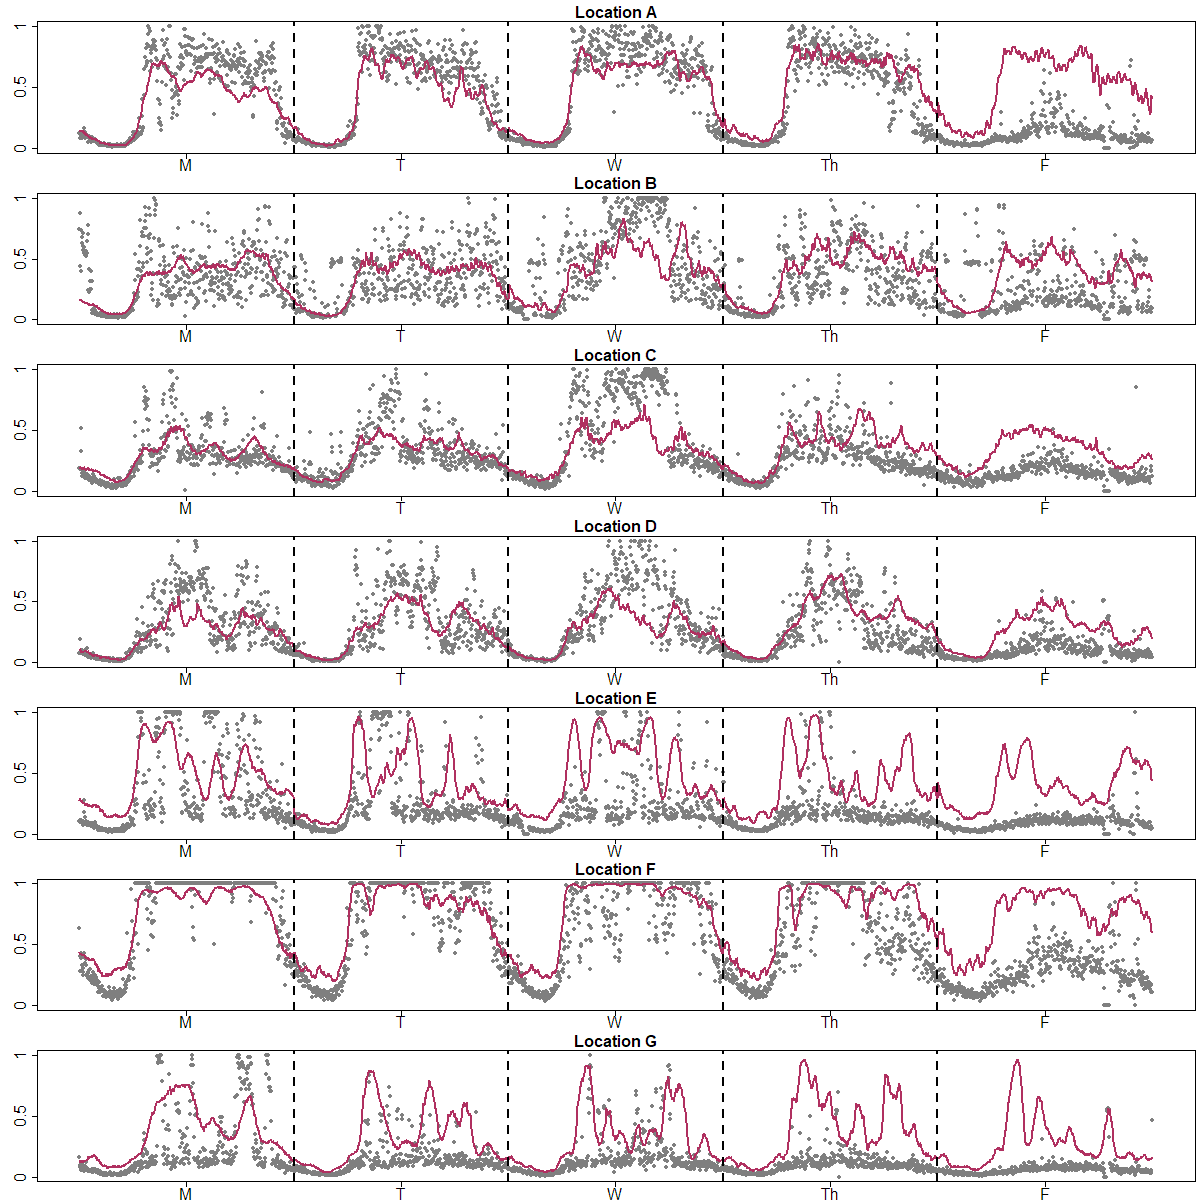
\includegraphics[width=\textwidth]{SEASESTPlots}
\label{fig:SEASESTPlots}
\end{figure}

\begin{figure}[htbp]
\caption{1-Step Ahead Density Forecasts for TAR Models}
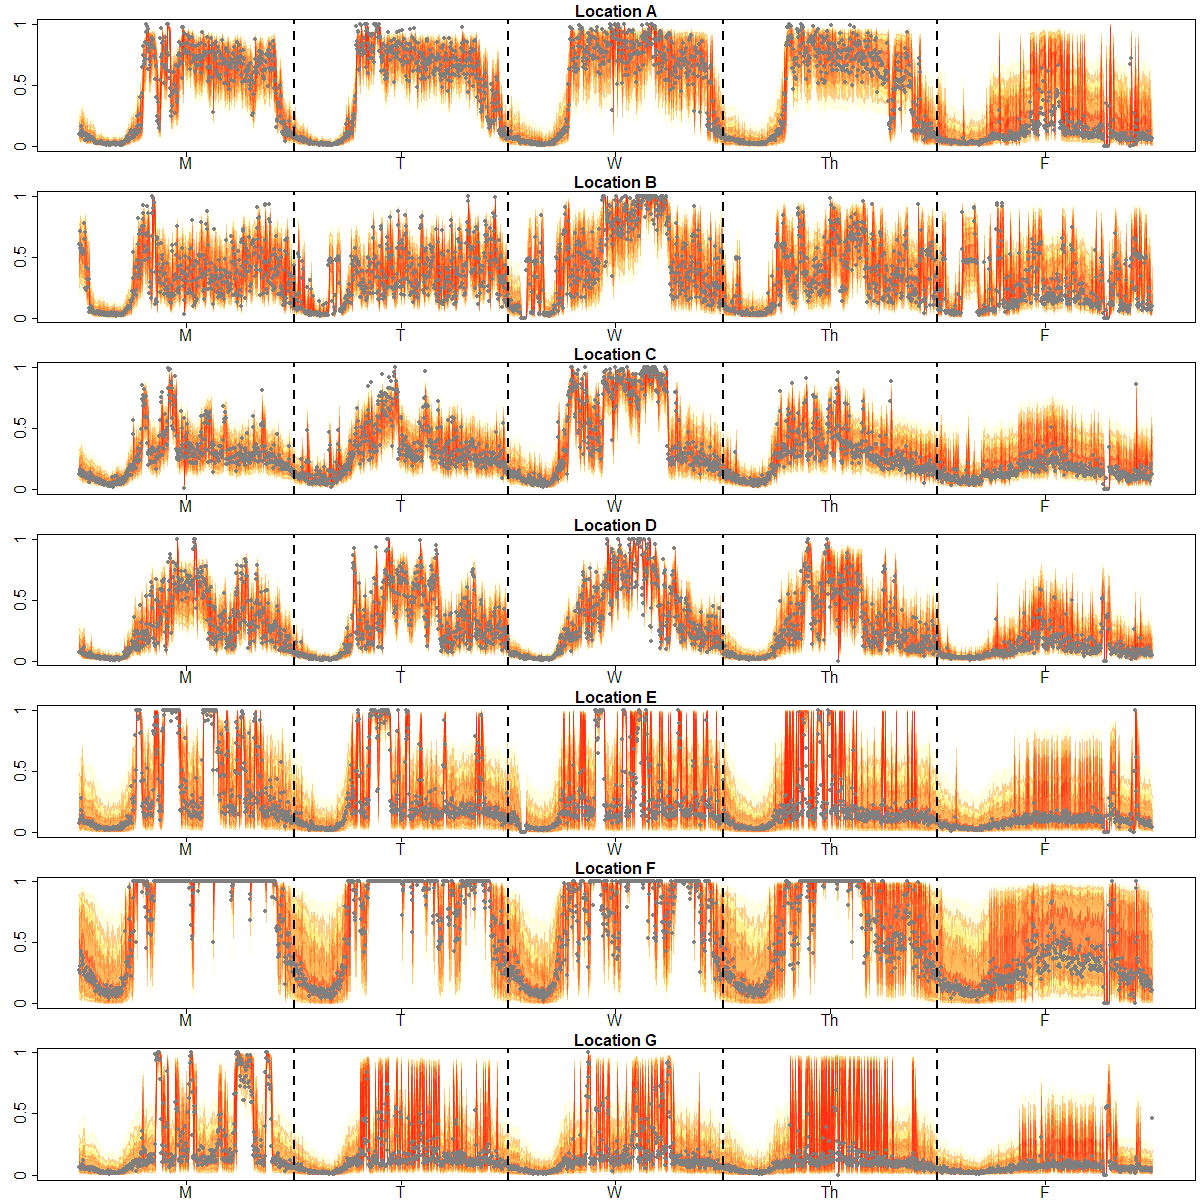
\includegraphics[width=\textwidth]{DENS1Plots}
\label{fig:DENS1Plots}
\end{figure}


\begin{figure}[htbp]
\caption{3-Step Ahead Density Forecasts for TAR Models}
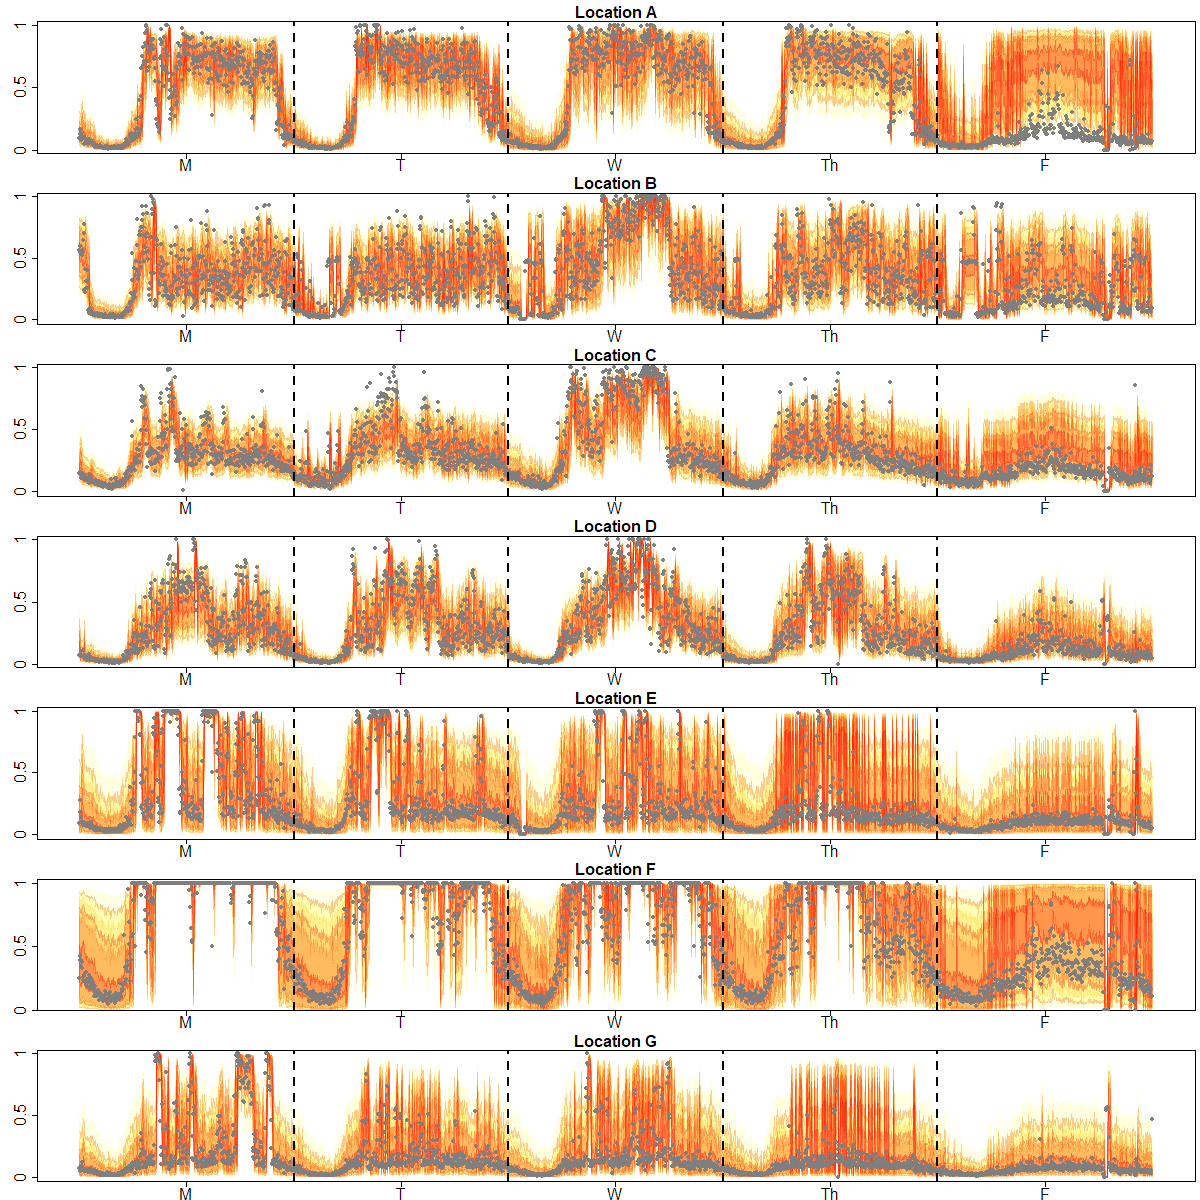
\includegraphics[width=\textwidth]{DENS3Plots}
\label{fig:DENS3Plots}
\end{figure}

\begin{figure}[htbp]
\caption{5-Step Ahead Density Forecasts for TAR Models}
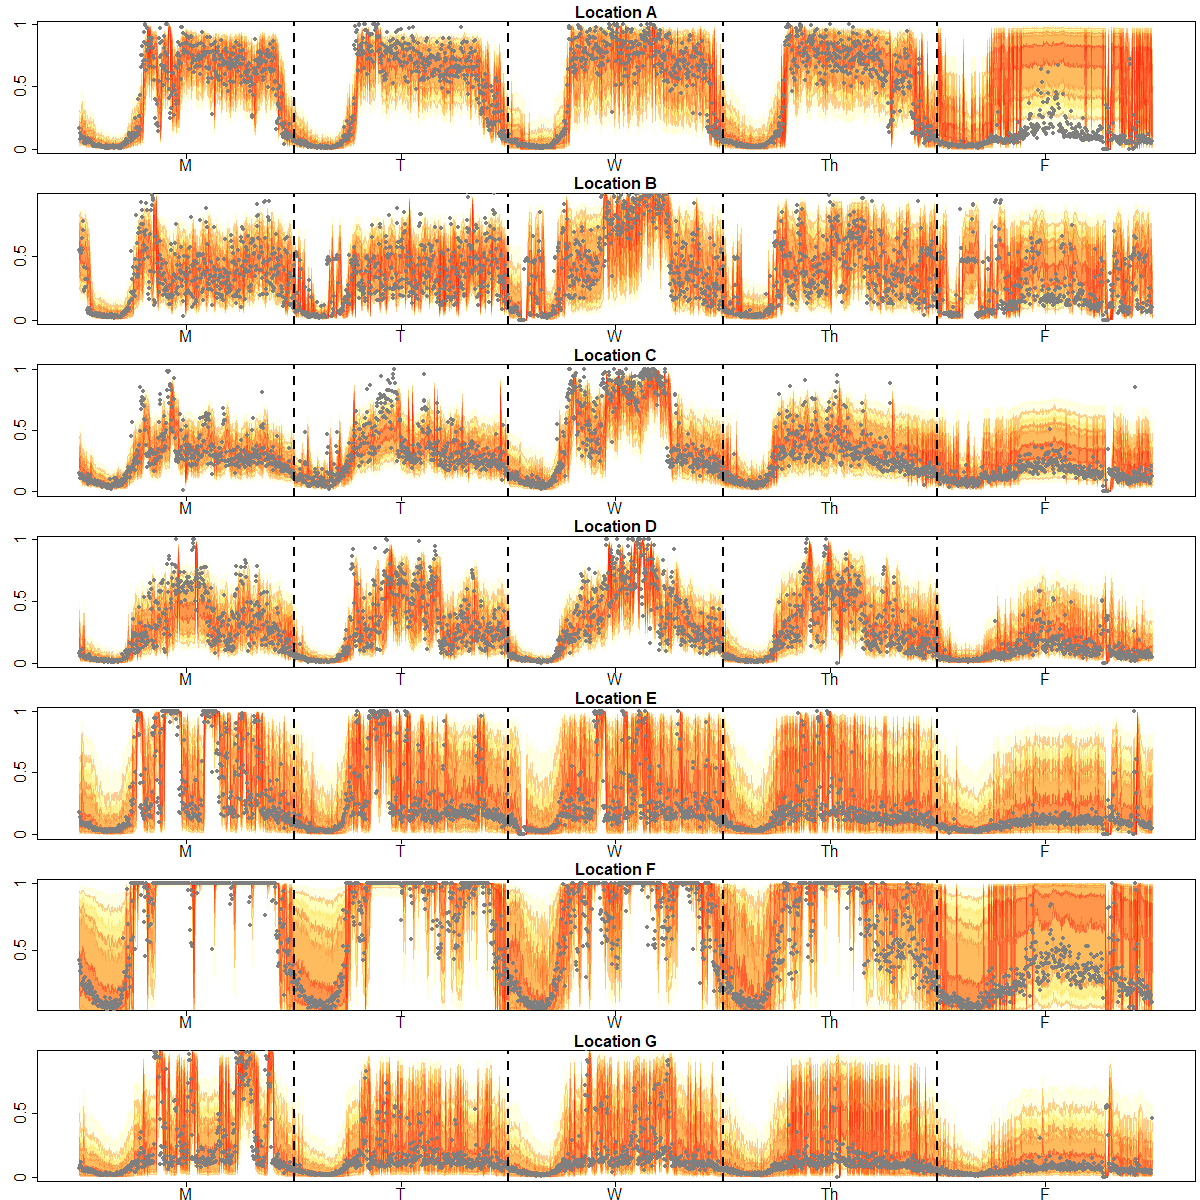
\includegraphics[width=\textwidth]{DENS5Plots}
\label{fig:DENS5Plots}
\end{figure}


Forecasts from both models over this period are evaluated using the mean absolute scaled forecast error (MASFE) metric from \cite{Hyndman2006}. The formulation of MASFE is found in Equation \ref{eq:trafficmase} where $\textrm{MAE}_{RW}(h)$ represents the mean absolute error from a $h$-specific naive random walk (RW) model over the fitting period where $\widehat{O}_{L,t}$ is the observed $O_{L,t-h}$. By scaling errors using $\textrm{MAE}_{RW}(h)$, TAR can be compared to SEAS and both can be compared to simple naive approaches. Whenever MASFE$(h)<1$, the model produces absolute forecast errors that are, on average, less than the forecast errors from a simple random walk model with no parameters.
\begin{equation}
\label{eq:trafficmase}
  \textrm{MASFE}(h)=\frac{1}{T_h}\sum\limits_{t=P+h}^{480}\left|\frac{O_{L,t}-\widehat{O}_{L,t}}{\textrm{MAE}_{RW}(h)}\right|
\end{equation}

Tables \ref{tab:trafficmase1}, \ref{tab:trafficmase3}, and \ref{tab:trafficmase5} compares final TAR and SEAS models for all days and locations at horizons $h\in \{1,3,5\}$, respectively. Multiple-regime TAR models consistently outperform SEAS profiles at all locations and days when forecasting 1-step ahead. For 3-step ahead forecasts, the SEAS model for Tuesday at location $C$ has a smaller MASFE, by a negligible amount. For 5-step ahead forecasts, more occurrences of SEAS producing forecasts, as good or better, than TAR are observed. The opposite pattern is exhibited for $h$-specific RW models. For 1-step ahead forecasts, MASFE$>1$ for many of the models. As the horizon $h$  increases, a clear advantage of using more complicated models (TAR and SEAS) to capture nonlinear and/or seasonal dynamics is notices. This is generally true except for locations $E$, $F$, and $G$ where traffic occupancies are considerably more difficult to model which is visually indicated by the wide credible regions in Figures \ref{fig:DENS1Plots}, \ref{fig:DENS3Plots}, and \ref{fig:DENS5Plots}.



\begin{table}[htbp]
\scriptsize
\centering
\caption{1-Step Ahead MASFE Forecast Comparison}
\begin{tabular}{c|rccccccc}
  \hline
  & & \multicolumn{7}{c}{Location}\\
  \cline{5-7}
Day & Model & A & B & C & D & E & F & G \\ 
  \hline
  \multirow{2}{*}{M} & TAR & 1.02 & 1.10 & 0.88 & 1.07 & 1.87 & 0.81 & 1.48 \\ 
  & SEAS & 1.80 & 1.47 & 1.15 & 1.43 & 4.02 & 1.57 & 3.66 \\ 
  \hline
  \multirow{2}{*}{T}  & TAR & 0.90 & 1.05 & 1.04 & 0.98 & 1.36 & 1.03 & 1.95 \\ 
  & SEAS & 1.35 & 1.36 & 1.22 & 1.46 & 3.36 & 1.65 & 3.29 \\ 
  \hline
   \multirow{2}{*}{W} & TAR & 1.04 & 1.11 & 0.91 & 0.97 & 2.27 & 1.86 & 1.55 \\ 
   & SEAS & 1.39 & 2.01 & 2.18 & 1.61 & 4.65 & 2.90 & 2.80 \\ 
  \hline
 \multirow{2}{*}{Th} & TAR & 0.93 & 0.89 & 0.82 & 0.92 & 1.48 & 1.52 & 1.83 \\ 
   & SEAS & 1.44 & 1.43 & 1.51 & 1.42 & 3.98 & 2.74 & 4.07 \\ 
  \hline
  \multirow{2}{*}{F} & TAR & 1.80 & 1.08 & 1.01 & 0.85 & 1.45 & 2.40 & 1.16 \\ 
   & SEAS & 4.77 & 2.23 & 1.98 & 1.83 & 4.37 & 6.24 & 3.78 \\ 
   \hline
\end{tabular}
\label{tab:trafficmase1}
\end{table}




\begin{table}[htbp]
\scriptsize
\centering
\caption{3-Step Ahead MASFE Forecast Comparison}
\begin{tabular}{c|rccccccc}
  \hline
    & & \multicolumn{7}{c}{Location}\\
  \cline{5-7}
Day & Model & A & B & C & D & E & F & G \\ 
  \hline
  \multirow{2}{*}{M} & TAR & 0.94 & 1.06 & 0.88 & 1.13 & 1.85 & 0.88 & 1.50 \\ 
   & SEAS & 1.36 & 1.17 & 0.93 & 1.14 & 2.91 & 1.19 & 2.57 \\ 
   \hline
  \multirow{2}{*}{T} & TAR & 0.87 & 1.04 & 0.96 & 1.03 & 1.46 & 1.15 & 1.21 \\ 
   & SEAS & 1.04 & 1.06 & 0.91 & 1.10 & 2.24 & 1.22 & 2.15 \\ 
   \hline 
  \multirow{2}{*}{W} & TAR & 1.09 & 1.15 & 1.10 & 0.99 & 1.75 & 2.00 & 1.26 \\ 
   & SEAS & 1.15 & 1.61 & 1.69 & 1.21 & 2.94 & 2.24 & 1.71 \\ 
   \hline
 \multirow{2}{*}{Th}  & TAR & 0.90 & 0.96 & 0.82 & 0.93 & 1.88 & 1.47 & 1.14 \\ 
   & SEAS & 1.15 & 1.09 & 1.14 & 1.03 & 2.69 & 1.96 & 2.68 \\ 
  \hline
  \multirow{2}{*}{F} & TAR & 3.04 & 1.09 & 1.00 & 0.66 & 1.14 & 2.47 & 0.92 \\ 
   & SEAS & 3.53 & 1.57 & 1.42 & 1.33 & 3.12 & 4.35 & 2.42 \\ 
   \hline
\end{tabular}
\label{tab:trafficmase3}
\end{table}




\begin{table}[htbp]
\scriptsize
\centering
\caption{5-Step Ahead MASFE Forecast Comparison}
\begin{tabular}{c|rccccccc}
  \hline
    & & \multicolumn{7}{c}{Location}\\
  \cline{5-7}
Day & Model & A & B & C & D & E & F & G \\ 
  \hline
  \multirow{2}{*}{M} & TAR & 0.94 & 0.99 & 0.89 & 1.12 & 1.97 & 0.86 & 1.68 \\ 
   & SEAS & 1.24 & 1.06 & 0.88 & 1.06 & 2.46 & 1.08 & 2.17 \\ 
  \hline
  \multirow{2}{*}{T}  & TAR & 0.81 & 1.05 & 0.95 & 1.00 & 1.47 & 1.13 & 1.15 \\ 
   & SEAS & 0.95 & 0.95 & 0.85 & 0.99 & 1.85 & 1.07 & 1.77 \\ 
  \hline
  \multirow{2}{*}{W}  & TAR & 1.02 & 1.12 & 1.04 & 0.99 & 1.67 & 1.94 & 1.26 \\ 
   & SEAS & 1.01 & 1.44 & 1.56 & 1.12 & 2.30 & 1.95 & 1.44 \\ 
  \hline
  \multirow{2}{*}{Th}  & TAR & 0.84 & 0.98 & 0.82 & 0.87 & 1.51 & 1.48 & 1.22 \\ 
   & SEAS & 1.05 & 1.03 & 1.07 & 0.94 & 2.13 & 1.73 & 2.24 \\ 
  \hline
  \multirow{2}{*}{F}  & TAR & 2.85 & 1.20 & 0.88 & 0.70 & 1.26 & 2.52 & 1.00 \\ 
   & SEAS & 3.07 & 1.48 & 1.33 & 1.19 & 2.59 & 3.82 & 2.01 \\ 
   \hline
\end{tabular}
\label{tab:trafficmase5}
\end{table}




\section{Conclusion}
Short-term forecasting of traffic occupancy is useful in real-time monitoring of a network. The nonlinearities present in the data make it difficult to get precise predictions. Daily traffic occupancy cycles between periods of free flow to periods of congestion. Threshold autoregressions capture many of these nonlinearities by using separate autoregressive processes to model dynamics for different states. Since occupancy is quality measure of traffic flow, this endogenous characteristic can characterize the regimes. 

The general estimation difficulties of TAR models lead users to fix the number of regimes prior to fitting the model. In this application to traffic occupancy, the number of thresholds $m$ is fixed and a high dimensional linear model matrix that nests many TAR models with regimes less than $m+1$ is constructed. Sparse estimation of the coefficients not only identifies the optimal number of regimes, but also selects the thresholds. After fixing the maximum autoregressive order $P$ and choosing the $m$ thresholds, we present a three step model building procedure that automates subset TAR$(P)$ selection. 

Using a metric scaled by the MAE of a naive random walk evaluated from the training period, advantages of TAR models over sparse periodic seasonal signals are discovered for forecasting 3, 9, and 15 minutes ahead. Nevertheless, there is room for improvement. The outlined posterior prediction projective method for subset selection of TAR requires the assumption that errors follow a \textit{normal} distribution with zero mean and constant variance. Although we estimate linear models using logit transformed data and capture some of the heteroskedasticity when we convert back to the original scale, it may be advantageous to modify the approaches with robust \textit{Student t} errors, within-regime homoskedasticity, or stochastic volatility models for the variance. 























